\chapter{Wikipedia multilingual graph}\label{wikipedia_multilingual_graph}
    In this section, I briefly describe the framework that can be used to build Wikipedia multilingual graphs. In general, it is not mandatory to use this part of the framework, since one can learn graph embeddings even without explicitly using the builder classes described in this chapter. However, a user might find this part of the framework useful because it provides him/her with some convenient classes and functions that allow to work with the Wikipedia multilingual graph in an intuitive way.
    
    Essentially, it facilitates the development of software applications and, in general, it makes a user's life easier because of the following reasons:
    \begin{itemize}
        \item It helps to save time, since the overall program’s flow of control is dictated by the framework, and not the caller.
        \item Since it is extensible, programmers can add specialized code to provide specific functionality.
        \item It is robust and efficient because it has been widely used and tested in several different settings.
        \item It eliminates the need to write a lot of repetitive code, thus allowing to work in a more efficient manner.
        \item Most importantly, it is completely integrated with the learning framework (described in chapter \ref{learning_framework}), meaning that a user does not have to worry about the conversion from the intuitive graph interface provided here and the more sophisticated, machine learning related input required by the learning framework.
    \end{itemize}
    \section{Downloading Wikipedia data}
        The first thing that you need if you want to start working with the Wikipedia multilingual graph is a practical and intuitive method to download Wikipedia data.
        \subsection{SQL dumps}
            The Wikimedia Foundation provides developers with a complete copy of all Wikimedia wikis. These snapshots are usually provided twice a month and, at the very least, monthly\footnote{\url{https://dumps.wikimedia.org/}.}. With regard to article text, data usually come embedded in XML. Instead, many raw database tables --- and, specifically, all the tables described in section \ref{wikipedia_database} --- are available in SQL form. In particular, the Wikimedia Foundation provides logical backups\footnote{A backup that reproduces table structure and data, without copying the actual data files. It is usually formed by queries that reconstruct tables and restore data. It is more flexible than a physical backup --- which copies the actual data files --- but can take substantially longer to restore.} --- i.e., dumps --- of its databases in order to facilitate the cloning of a particular table: these files contain metadata from Wikipedia describing its structure and organization.
            
            In order to get the fundamental information to build a multilingual graph of Wikipedia, one only needs to have access to SQL tables provided by Wikimedia Foundation: they contain all the information related to links between pages, titles, \textquote{is-a} relationships between categories, redirects, etc. Text from the Wikipedia pages is not necessary to build a graph: XML files can be ignored for the moment.
            
            After few initial experiments, I abandoned the idea to work directly with the SQL dumps provided by Wikipedia. Indeed:
            \begin{itemize}
                \item Downloading dumps of many SQL tables and restore them is a very time consuming and computationally expensive operation. In fact, a dump is not intended as a fast solution for backing up a large amount of data: when a database is huge --- as the Wikipedia one is --- restoring the data can be very slow because replaying the SQL statements involves disk input/output for insertion, index creation, and so on. Restoring a Wikipedia SQL dump can take literally days.
                \item Furthermore, when the goal is to build a multilingual graph, one needs to download a number of tables for each language: the amount of data to manage is very large, and not everybody has enough resources for such a task. For example, the uncompressed pagelinks dump file (the pagelinks is the biggest table in a Wikipedia database) of the English Wikipedia is about 37 gigabytes, and the related table size is estimated to be 200 gigabytes. However, most of the data contained in these tables are not useful to build a multilingual graph.
            \end{itemize}
        \subsection{Wikipedia downloader}\label{wikipediadownloader}
            In order to overcome these issues, I have designed a standalone Python module --- called \monospace{wikipedia\_downloader} --- that simplifies the download and decompression of Wikipedia dumps, and helps selecting only useful rows or filtering useless columns. Specifically, it provides users with:
            \begin{itemize}
                \item A method for downloading and decompressing on-the-fly a SQL dump of a table. In this way, multiple tables can be dynamically downloaded through a Python script, thus integrating this functionality with the remaining part of the application.
                \item A method for selectively downloading a table. In other words, it is a method that emulates the functionality of a typical \textquote{\monospace{SELECT [\dots] FROM [\dots] WHERE [\dots]}} SQL statement, and, at the same time, download and save only what is strictly required by the user.
            \end{itemize}
            
            Here is a summary of each method's functionality and a complete description of parameters and outputs.
            \begin{functiondoc}{wikipedia\_downloader}{download\_sql\_dump}{lang, table, dump="latest", target\_dir="."}
                \begin{functiondescription}
                    Download and decompress on-the-fly a Wikipedia table SQL dump, and save results on disk.
                    
                    Files are downloaded directly from the Wikimedia servers, where the number of per-IP connections is capped to two (you should not try to evade these limits, otherwise you may be blocked).

                    Files are saved in the target directory with their original name, whose format is \monospace{[lang]wiki-[dump]-[table].sql}.
                \end{functiondescription}

                \begin{functionparameters}
                    \item[lang] string
                    
                    Language code that represents the Wikipedia name. Each Wikipedia has a code (see \url{http://en.wikipedia.org/wiki/List_of_Wikipedias\#Wikipedia_edition_codes}), which is used as a subdomain below \url{http://www.wikipedia.org/}. The codes represent the language codes defined by ISO 639-1 and ISO 639-3 (see \url{http://www.iso.org/iso-639-language-codes.html}).
                    \item[table] string
                    
                    Name of the table to be downloaded. Possible values are \inlinecode{"pagelinks"}, \inlinecode{"redirect"}, \inlinecode{"page"} etc. Some tables may not be available on all wikis. In general, the available database tables can be found at \url{https://meta.wikimedia.org/wiki/Data_dumps/What\%27s_available_for_download\#Database_tables}.
                    \item[dump] string, default \inlinecode{"latest"}
                    
                    Dump version to be used when downloading a table. This value can be either \inlinecode{"latest"} (default value, it represents the last available dump) or a string indicating the dump creation date (formatted as YYYYMMDD). For example, one may use \inlinecode{"20190101"}, \inlinecode{"20190320"}, etc. Available dumps can be found at \monospace{http://dumps.wikimedia.org/[lang]wiki} (replace \monospace{[lang]} with the language code that represents the desired Wikipedia version).
                    
                    \item[target\_dir] string, default \inlinecode{"."}
                    
                    File path where the downloaded and uncompressed SQL dump will be stored.
                \end{functionparameters}
                
                \begin{functionoutput}
                    \inlinecode{None}
                \end{functionoutput}
                
                \begin{functionexample}
import wikipedia_downloader as wpd
wpd.download_sql_dump("en", "pagelinks",
                      dump="20190101",
                      target_dir="./dumps")
                \end{functionexample}
            \end{functiondoc}
            \begin{functiondoc}{wikipedia\_downloader}{get\_dataframe}{lang, table, dump="latest", select=None, where=None}
                \begin{functiondescription}
                    Build a \monospace{pandas.DataFrame} from a SQL dump of a Wikipedia table.
                    
                    Unwanted columns and records can be filtered out using a SQL-like interface. In this way, a user can download and store only data that is strictly required, thus possibly saving much space.
                \end{functiondescription}
                
                \begin{functionparameters}
                    \item[lang] string
                    
                    Language code (defined by ISO 639-1 and ISO 639-3) that represents the Wikipedia name.
                    \item[table] string
                    
                    Name of the table to be downloaded.
                    \item[dump] string, default \inlinecode{"latest"}
                    
                    Dump version to be used when downloading a table. This value can be either \inlinecode{"latest"} (default value, it represents the last available dump) or a string indicating the dump creation date (formatted as YYYYMMDD).
                    
                    \item[select] array, default \inlinecode{None}
                    
                    Columns to be kept.
                    
                    The array contains the names of the columns to be selected. The default value (\inlinecode{None}) indicates that all the table columns must be selected.
                    
                    Columns of each table can be found in the related manuals (a complete list of table manuals can be found at \url{http://www.mediawiki.org/wiki/Category:MediaWiki_database_tables}).
                    \item[where] dictionary, default \inlinecode{None}
                    
                    Functions used to filter records.
                    
                    The dictionary contains a key for every column used to filter records, where the name of the key is equal to the related column. Each key is associated with a filter function, that can be defined by the user. The filter function is given the column value of the record (the one associated with the key), and returns true if the record should be kept and false otherwise.
                \end{functionparameters}
                
                \begin{functionoutput}
                    \monospace{pandas.DataFrame} object (see \url{http://pandas.pydata.org}). It is a tabular data structure with labeled columns. It can be thought of as a dictionary-like container for series of values, where each series is a column of the original SQL table.
                \end{functionoutput}

                \begin{functionexample}
import wikipedia_downloader as wpd
select = ["page_id", "page_namespace", "page_title"]
where = {"page_namespace": lambda x: x == 14}
df = wpd.get_dataframe("en", "page",
                       dump="20190101",
                       select=select,
                       where=where)
                \end{functionexample}
            \end{functiondoc}
            
            Pandas\footnote{\url{http://pandas.pydata.org/}.} is a Python open source library that provides many data structures and data analysis tools. It is one of the most preferred and widely used tools in data science, if not the most used one. I have decided to rely on this library because its \monospace{DataFrame} class is much easier to work with in comparison to work with lists and/or dictionaries, since it provides column names in an R-style syntax. Also, this library has a lot of built in functions for a many common data processing applications (for example, datasets can be merged and joined in a very efficient way). Finally, Pandas is highly optimized for performance, with critical code written in C. Pandas flexibility and built in functions allow users to further process the downloaded tables in a standard and efficient way.
    \section{Building category and article graphs}
        The framework provides users with a method to build category graphs --- i.e., semi-hierarchical graphs formed by the categories of a specific Wikipedia version --- and article graphs --- i.e., highly connected graphs formed by articles of a wiki.
        
        Graphs are implemented using a very fast and efficient library for network analysis: it allows to easily run many standard algorithms and conveniently display graphs using a variety of output formats. In general, the provided interface is flexible enough to allow users to write their own functions based on category or article graphs.
        
        The framework also includes some utility functions that can be used to modify such graphs, for example to remove unwanted categories or links.
        \subsection{Graph-tool}
            All the graph structures used by the framework are implemented using graph-tool\footnote{\url{http://graph-tool.skewed.de/}.}: it is a Python package for the creation, manipulation, and study of the structure, dynamics, and functions of graphs. Contrary to more famous Python modules with similar functionality (for example, NetworkX\footnote{\url{http://networkx.github.io/}.}), the core data structures and algorithms are written in C++, thus making this tool faster than others.
            
            Moreover, graph-tool improves systematically its performance when it runs in multi-core architectures\footnote{\url{http://graph-tool.skewed.de/performance}.}, and it is optimized even from a memory usage point of view: when you deal with large graphs (such as the ones related to Wikipedia), using this module in Python is basically a must.
            
            Finally, graph-tool provides many useful features for manipulation, visualization and statistical analysis of graphs. Here are the most important for the development of the framework:
            \begin{itemize}
                \item It supports arbitrary vertex, edge or graph properties, meaning that nodes and edges can be virtually \textquote{anything}.
                \item It allows to efficiently filter vertices and edges on-the-fly --- i.e., vertices and edges can be temporary masked and then easily recovered. This functionality is implemented through the GraphView\footnote{\url{https://graph-tool.skewed.de/static/doc/quickstart.html\#graph-views}.} class: it represents a filtered \textquote{view} of a graph, and behaves as an independent graph object, which shares the underlying data with the original graph.
                \item It includes many implemented centrality-related algorithms (such as PageRank, betweenness centrality, etc.) and topological algorithms (such as connected components).
            \end{itemize}
        \subsection{Category graph builder}\label{categorygraphbuilder}
            The framework includes a helpful class that allows to automatically build the category graph of a Wikipedia version: \monospace{CategoryGraphBuilder}. In particular, this class provides users with a simple interface for building a  \monospace{graph\_tool.Graph}\footnote{\url{http://graph-tool.skewed.de/static/doc/graph_tool.html\#graph_tool.Graph}.} that represents a category graph of some Wikipedia version.
            
            This class is implemented using the Builder design pattern \cite{Gamma}, whose goal is to separate the object building process from the object representation. In this way, a user of the framework does not need to know how the graph tool library works, since he/she only needs to know how to use the interface of the builder. Moreover, the builder pattern allows a user to construct the object step by step, thus controlling which operations are performed on the graph.
            
            Here is a summary of the class' functionality and a complete description of methods and parameters.
            \begin{classdoc}{CategoryGraphBuilder}{Class that provides an interface which allows to build a category graph of a specific Wikipedia version.}
                \item \begin{classmethod}{CategoryGraphBuilder}{lang, dump="latest", cache\_dir="."}
                
                    \begin{functiondescription}
                        Constructor of the class. It instantiates a new \monospace{CategoryGraphBuilder} object. Such object can be used to build the category graph of a specific Wikipedia version.
                    \end{functiondescription}
                    
                    \begin{functionparameters}
                        \item[lang] string
                        
                        Language code (defined by ISO 639-1 and ISO 639-3) that represents the Wikipedia version from which the category graph has to be built.
                        \item[dump] string, default \inlinecode{"latest"}

                        Dump version to be used when building the category graph. This value can be either \inlinecode{"latest"} (default value, it represents the last available dump) or a string indicating the dump creation date (formatted as YYYYMMDD).
                        \item[cache\_dir] string, default \inlinecode{"."}
                    
                        File path where the builder can search for tables that have been already downloaded. If a table needed by the builder is already in the cache then it is not downloaded again. Cache support two types of files:
                        \begin{enumerate}
                            \item SQL dumps of the tables --- i.e., those that can be downloaded with the \monospace{download\_sql\_dumps} function.
                            \item Pickles objects of the tables --- i.e., serialization objects that can be obtained from dataframes (such as those returned by the \monospace{get\_dataframe}) using the \monospace{pandas.DataFrame.to\_pickle} function.
                        \end{enumerate}
                        Supported file names are \monospace{[lang]wiki-[dump]-[table].(sql|pkl)}.
                    \end{functionparameters}
                \end{classmethod}
                \item \begin{classmethod}{remove\_hidden\_categories}{}
                
                    \begin{functiondescription}
                        Remove all the hidden categories from the category graph.
                        
                        Unlike normal categories, hidden categories are hidden from users and not displayed in a Wikipedia page.
                    \end{functiondescription}
                    
                    \emptyfunctionparameters{}
                    
                    \begin{functionoutput}
                        The \monospace{CategoryGraphBuilder} object itself. Such returned value is useful when one wants to make many subsequent calls of methods of the same object.
                    \end{functionoutput}
                \end{classmethod}
                \item \begin{classmethod}{remove\_administration\_categories}{}
                
                    \begin{functiondescription}
                        Remove all the administration categories from the category graph.
                        
                        This method is language-dependent: it is not implemented for every language, and therefore it may not work on some graphs. For the moment, it works only with the English and Italian Wikipedia.
                        
                        A user can extend the \monospace{CategoryGraphBuilder} class and implement this method for other languages.
                    \end{functiondescription}
                    
                    \emptyfunctionparameters{}
                    
                    \begin{functionoutput}
                        The \monospace{CategoryGraphBuilder} object itself.
                    \end{functionoutput}
                \end{classmethod}
                \item \begin{classmethod}{remove\_categories}{categories}
                
                    \begin{functiondescription}
                        Remove from the category graph all the categories indicated in the input list.
                        
                        This function can be used to remove specific categories, no matter how they are found out: it is a flexible method for a user to remove generic categories from the graph.
                    \end{functiondescription}
                    
                    \begin{functionparameters}
                        \item[categories] iterable
                        
                        Iterable object that contains the IDs of the categories to be removed from the category graph. Every iterable is accepted, no matter if it is a list, a set, etc. Even a generator function can be used (see example below).
                    \end{functionparameters}
                    
                    \begin{functionoutput}
                        The \monospace{CategoryGraphBuilder} object itself.
                    \end{functionoutput}
                    
                    \begin{functionexample}
def useless_categories():
    while(some condition):
        // find a useless category identified by ID
        yield ID
other_useless_categories = [35, 12, 441995]

(builder.remove_categories(useless_categories())
        .remove_categories(other_useless_categories))
                    \end{functionexample}
                \end{classmethod}
                \item \begin{classmethod}{remove\_redirects}{}
                
                    \begin{functiondescription}
                        Remove from the category graph all the redirects between categories.
                        
                        Redirects data are contained in different tables (some are store in the pagelinks table, other in the redirects table, depending on the age of the information): this function helps the user to deal with these issues. In general:
                        \begin{enumerate}
                            \item Categories that redirect to other categories are ignored.
                            \item Categories that are target of redirect categories inherit their \textquote{is-a} relationships (that is, A is-a B, where B redirects to C, becomes A is-a C).
                        \end{enumerate}
                    \end{functiondescription}
                    
                    \emptyfunctionparameters{}
                    
                    \begin{functionoutput}
                        The \monospace{CategoryGraphBuilder} object itself.
                    \end{functionoutput}
                \end{classmethod}
                \item \begin{classmethod}{get\_graph}{}
                
                    \begin{functiondescription}
                        Return to the client the graph that has been built.
                    \end{functiondescription}
                    
                    \emptyfunctionparameters{}
                    
                    \begin{functionoutput}
                        The \monospace{graph\_tool.Graph} object that has been built by the \monospace{CategoryGraphBuilder} object and represents the Wikipedia category graph.
                    \end{functionoutput}
                    
                    \begin{functionexample}
builder = CategoryGraphBuilder("en")
graph = (builder.remove_redirects()
                .remove_hidden_categories()
                .remove_categories([4, 1995])
                .get_graph())
                    \end{functionexample}
                \end{classmethod}
            \end{classdoc}
            \subsubsection{Category graph}\label{categorygraph}
                The \monospace{CategoryGraphBuilder} class encapsulates creating and assembling the parts of a complex Wikipedia category graph. It is implemented by keeping an internal representation of the final graph: the result can be accessed by the client only after using the \monospace{get\_graph} method.
                
                The object of type \monospace{graph\_tool.Graph} returned by the \monospace{get\_graph} method represents the Wikipedia category graph. In particular, every vertex has two properties:
                \begin{itemize}
                    \item The ID of the category page --- i.e., the number that uniquely identifies a page belonging to a certain Wikipedia version.
                    \item The title of the category page --- i.e., the name of the category that uniquely identifies a page belonging to category namespace of a certain Wikipedia version.
                \end{itemize}
                These properties are implemented using the \monospace{graph\_tool.VertexpropertyMap} class\footnote{\url{https://graph-tool.skewed.de/static/doc/graph_tool.html\#graph_tool.VertexPropertyMap}.}. Here is an example of how they can be accessed\footnote{The vertex index should not be confused with the vertex ID. Indeed, the former is a number used by \monospace{grahp\_tool} in its internal representation, the latter is a number used in Wikipedia to uniquely identify pages. Specifically, in \monospace{graph\_tool} each vertex in a graph has an unique index, which is always between 0 and N-1, where N is the number of vertices.}:
                \begin{example}
v = graph.vertex(0) // vertex with index 0
id_v = graph.vertex_properties["id"][v] // vertex ID
name_v = graph.vertex_properties["name"][v] // vertex name
                \end{example}
                
                All the edges of such graph represent inheritance and generalization/specialization (is-a) relationships between categories belonging to the same Wikipedia version.
            \subsubsection{Network usage}
                The \monospace{CategoryGraphBuilder} class makes use of the \monospace{wikipedia\_downloader} module (defined and presented in section \ref{wikipediadownloader}) to download the appropriate tables from the Wikipedia servers. Therefore, this class cannot be used when the user is not connected to the Internet.
                
                There is an exception, though. If all the tables needed by the methods of \monospace{CategoryGraphBuilder} are already stored in the cache directory, then there is no need to be connected to the Internet. Indeed, the framework checks whether or not files have already been downloaded: if this has not been the case, \monospace{CategoryGraphBuilder} uses \monospace{wikipedia\_downloader} to download the needed tables, otherwise it simply use stored data. In particular, \monospace{CategoryGraphBuilder} may need:
                \begin{itemize}
                    \item The \emph{categorylinks} table. Specifically, the table must contain at least the columns \emph{cl\_from}, \emph{cl\_to} and \emph{cl\_type}.
                    \item The \emph{page} table. Specifically, the table must contain at least the columns \emph{page\_id}, \emph{page\_namespace}, \emph{page\_title} and \emph{page\_is\_redirect}.
                    \item The \emph{pagelinks} table. Specifically, the table must contain at least the columns \emph{pl\_from}, \emph{pl\_from\_namespace}, \emph{pl\_namespace} and \emph{pl\_title} (at the moment, these are all the possible columns of this table).
                    \item The \emph{redirect} table. Specifically, the table must contain at least the columns \emph{rd\_from} and \emph{rd\_title}.
                \end{itemize}
                More details about these tables and the related columns can be found in section \ref{wikipedia_database}.
        \subsection{Article graph builder}\label{articlegraphbuilder}
            The framework also provides users with a class that allows to automatically build the article graph of a Wikipedia version: \monospace{ArticleGraphBuilder}. In particular, this class provides users with a simple interface for building a  \monospace{graph\_tool.Graph} that represents highly connected graphs formed by articles of a wiki.
            
            As in the case of \monospace{CategoryGraphBuilder}, this class is implemented using the Builder design pattern, which allows a user to construct the object step by step.
            
            Here is a description of the class' functionality. Since this class is very similar to \monospace{CategoryGraphBuilder}, only a brief summary is given. For more details, refer to section \ref{categorygraphbuilder}.
            \begin{classdoc}{ArticleGraphBuilder}{Class that provides an interface which allows to build the graph of all the articles of a specific Wikipedia version. It separates the construction of the complex graph object from its representation, thus providing the user with a flexible solution for building different article graphs.}
                \item \begin{classmethod}{ArticleGraphBuilder}{lang, dump="latest", cache\_dir="."}
                
                    \begin{functiondescription}
                        Constructor of the class. It instantiates a new \monospace{ArticleGraphBuilder} object. Such object can be used to build the article graph of a specific Wikipedia version.
                    \end{functiondescription}
                    
                    \begin{functionparameters}
                        \item[lang] string
                        
                        Language code that represents the Wikipedia version from which the article graph has to be built.
                        \item[dump] string, default \inlinecode{"latest"}

                        Dump version to be used when building the article graph (\inlinecode{"latest"} or a string formatted as YYYYMMDD).
                        \item[cache\_dir] string, default \inlinecode{"."}
                    
                        File path where the builder can search for tables that have been already downloaded. Cache support two types of files: SQL dumps and pickles objects of the tables. Supported file names are \monospace{[lang]wiki-[dump]-[table].(sql|pkl)}.
                    \end{functionparameters}
                \end{classmethod}
                \item \begin{classmethod}{remove\_articles}{articles}
                
                    \begin{functiondescription}
                        Remove from the article graph all the articles indicated in the input iterable object.
                    \end{functiondescription}
                    
                    \begin{functionparameters}
                        \item[articles] iterable
                        
                        Iterable object that contains the IDs of the articles to be removed from the article graph.
                    \end{functionparameters}
                    
                    \begin{functionoutput}
                        The \monospace{CategoryGraphBuilder} object itself.
                    \end{functionoutput}
                \end{classmethod}
                \item \begin{classmethod}{remove\_redirects}{}
                
                    \begin{functiondescription}
                        Remove from the article graph all the redirects between articles.
                    \end{functiondescription}
                    
                    \emptyfunctionparameters{}
                    
                    \begin{functionoutput}
                        The \monospace{ArticleGraphBuilder} object itself.
                    \end{functionoutput}
                \end{classmethod}
                \item \begin{classmethod}{get\_graph}{}
                
                    \begin{functiondescription}
                        Return to the client the graph that has been built.
                    \end{functiondescription}
                    
                    \emptyfunctionparameters{}
                    
                    \begin{functionoutput}
                        The \monospace{graph\_tool.Graph} object that has been built by the \monospace{ArticleGraphBuilder} object and represents the Wikipedia article graph.
                    \end{functionoutput}
                    
                    \begin{functionexample}
builder = ArticleGraphBuilder("en")
graph = (builder.remove_redirects()
                .remove_articles([12, 3, 93])
                .get_graph())
                    \end{functionexample}
                \end{classmethod}
            \end{classdoc}
            For the moment, the \monospace{ArticleGraphBuilder} class does not have much functionality, since I have made only few experiments with article graphs. However, it can be easily extended and new methods can be added by future users. For example, one may want to remove all the articles which do not have any hyperlink or do not belong to any category.
            \subsubsection{Article graph}
                The \monospace{ArticleGraphBuilder} is an interface that can be used to build a graph of all the articles of a wiki. In particular, this graph is an object of type \monospace{gfraph\_tool.Graph} and it has the following characteristics:
                \begin{itemize}
                    \item The edges of this graph represent the hyperlinks that allow users to jump to information related to the article they are reading, greatly improving Wikipedia's usefulness.
                    \item Each vertex of the graph represents an article. Moreover, each vertex has two properties: ID and name --- i.e., unique identifier and title of the page. These properties are implemented through the use of the \monospace{graph\_tool.VertexPropertyMap} class (see section \ref{categorygraph} for more details and an example). The vertex ID should not be confused with the vertex index.
                \end{itemize}
            \subsubsection{Network usage}    
                As in the case of \monospace{CategoryGraphBuilder}, the network is needed if the necessary tables are not stored in the cache directory (either in SQL dumps form or in pickles object form). Tables which are not found in the cache directory are downloaded using the \monospace{wikipedia\_downloader} module described in section \ref{wikipediadownloader}.
                
                The tables that are needed by the \monospace{ArticleGraphBuilder} to successfully build the Wikipedia article graph are: \emph{page}, \emph{pagelinks} and \emph{redirect}. If a user create new methods or overwrite the existing ones then more tables may need to be added to the list.
    \section{Going multilingual}
        Once monolingual graphs have been built (using one of the classes described in sections \ref{categorygraphbuilder} and \ref{articlegraphbuilder}), one can merge them and form a multilingual graph.
        
        Each Wikipedia version provides a table called \emph{langlinks}. It contains the inter-language links: they are links from one Wikipedia version to an equivalent page in another language. These connections can help a lot to find vertices belonging to different graph that can be merged. However, merging multiple different monolingual graphs can be very difficult, even if one has the langlinks table.
        
        This section presents the challenges one has to face when merging multiple monolingual graphs. Moreover, it describes which practical tools can be used to build a multilingual graph and how users can extend them. The last part of this section describes a possible solution to the merging problem, discussing pros and cons.
        \subsection{Challenges in graph merging}\label{challenges_merging}
            Merging several monolingual graphs using langlinks tables can be very challenging, no matter which graphs one is dealing with (article or category graphs). Here are some common issues:
            \begin{itemize}
                \item No data is stored for a vertex (missing values). In general, this issue can have a significant effect on the conclusions that can be drawn from the data. The question to be answered is whether there is a vertex in other monolingual graphs which represents the same concept. This is not a problem if the concept is described only in a single Wikipedia version, but it is not easy to know whether or not this is the case.
                \item Information contained in langlinks tables may be simply wrong. Indeed, Wikipedia is based on a model of openly editable content, and everybody can edit data in a malicious manner (for example, by adding material that is nonsensical).
                \item Data may be inconsistent when comparing different Wikipedia versions. Indeed, each Wikipedia version is curated in an independent way by a different community: sometimes, inter-language links are incoherent and point to two different vertices.
            \end{itemize}
            In general, many of the issues are caused by the fact that the same concept is represented with a single page in one language, and with multiple pages in another language, thus confusing the users which have to create inter-language links between different wikis. An example is shown in figure \ref{langlinks_problems}.
            
            \begin{figure}
                \centering
                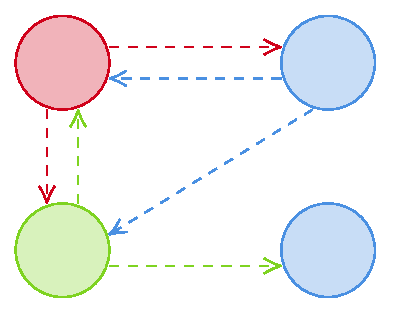
\includegraphics[width=0.5\textwidth]{images/langlinks_problems.pdf}
                \caption{When one tries to merge multiple monolingual graphs, he/she may have to face some issues. Here is an example in which different Wikipedia communities (red, green and blue) disagree on how some vertices should be merged (dotted arrows represent inter-language links). While in this situation one can conclude that the green community is wrong because other communities have found an agreement, there can be more difficult situations in which it is not completely clear what to do.}
                \label{langlinks_problems}
            \end{figure}
        \subsection{Multilingual graph builder}\label{multilingualbuilder}
            The framework provides users with a class that allows to dynamically build multilingual graphs from monolingual graphs: \monospace{MultilingualGraphBuilder}.
            
            As in the case of monolingual category and article graphs, this class relies on the graph-tool library, because of its high performance and low memory requirements. Specifically, \monospace{MultilingualGraphBuilder} provides users with a simple interface for building a \monospace{graph\_tool.Graph} that represents a multilingual graph of some Wikipedia version (related to either categories or articles).
            
            This class is implemented using the Builder design pattern. In this way, a user can dynamically construct the Wikipedia multilingual graph, choosing at each step which operation should be performed.
            
            Here is a summary of the class' functionality. Many details are similar to those presented in sections \ref{categorygraphbuilder} and \ref{articlegraphbuilder} and are therefore described only briefly.
            \begin{classdoc}{MultilingualGraphBuilder}{Class that provides an interface which allows to build a multilingual graph of categories or articles belonging to different Wikipedia versions.}
                \item \begin{classmethod}{MultilingualGraphBuilder}{dump="latest", cache\_dir=".", cache\_size=10}
                
                    \begin{functiondescription}
                        Constructor of the class. It instantiates a new \monospace{MultilingualGraphBuilder} object. Such object can be used to build the multilingual graph of categories or articles belonging to several wikis.
                    \end{functiondescription}
                    
                    \begin{functionparameters}
                        \item[dump] string, default \inlinecode{"latest"}

                        Dump version to be used when building the multilingual graph. This value can be either \inlinecode{"latest"} (default value, it represents the last available dump) or a string indicating the dump creation date (formatted as YYYYMMDD).
                        
                        All the category or article graphs to be merged must have been built with data coming from the same dump.
                        \item[cache\_dir] string, default \inlinecode{"."}
                    
                        File path where the builder can save data that might be used again. If the builder does not find the information it is looking for, then it will download it from Wikipedia servers using the \monospace{wikipedia\_downloader} module.
                        
                        Files are saved in cache using an internal format and policy that can change in the future: the users should not try to manually add and/or remove files from cache while building the multilingual graph.
                        \item[cache\_size] number, default \inlinecode{10}
                    
                        The amount of physical memory that the cache can use (in gigabytes).
                    \end{functionparameters}
                \end{classmethod}
                \item \begin{classmethod}{add\_graphs}{graphs}
                
                    \begin{functiondescription}
                        Add to the multilingual graph all the monolingual graphs indicated in the input list. This function can be used to incrementally add new category or article graphs to the multilingual graph that the user is building.
                        
                        There is a requirement that must be satisfied, though: all the graphs indicated in the input list --- as well those that were previously added to the multilingual graph --- must have been built with data coming from the same Wikipedia dump. In fact, there can be inter-language links that point to non-existing pages, if this condition does not hold.
                        
                        The same monolingual graph cannot be added twice.
                    \end{functiondescription}
                    
                    \begin{functionparameters}
                        \item[graphs] iterable of \monospace{graph\_tool.Graph} objects
                        
                        Iterable object that contains category or article graphs of type \monospace{graph\_tool.Graph}. These kind of graphs can be obtained using, respectively, the \monospace{CategoryGraphBuilder} and \monospace{ArticleGraphBuilder} classes. Every iterable is accepted, no matter if it is a list, a set, etc. Even a generator function can be used (see example below).
                    \end{functionparameters}
                    
                    \begin{functionoutput}
                        The \monospace{MultilingualGraphBuilder} object itself.
                    \end{functionoutput}
                    
                    \begin{functionexample}
def get_category_graphs():
    for lang in ("en", "it", "de"):
        // Build category graph
        builder = CategoryGraphBuilder(lang)
        graph = (builder.remove_redirects()
                        .get_graph())
        yield graph

builder = MultilingualGraphBuilder()
builder = builder.add_graphs(get_category_graphs())
                    \end{functionexample}
                \end{classmethod}
                \item \begin{classmethod}{merge}{merging\_strategy=None}
                
                    \begin{functiondescription}
                        Merge vertices of the multilingual graph.
                        
                        In general, the \monospace{MultilingualGraphBuilder} class keeps track of inter-language links between vertices that belong to different monolingual graphs. Inter-language links indicate that two vertices may represent the same concept and therefore could be merged. When the user calls the merge method, some vertices (possibly those which are connected by inter-language links, but this is not a requirement) are merged into a single vertex, according to a \emph{merging strategy}.
                        
                        Another effect of using this method is that all the inter-language links are converted to normal edges: no matter how vertices are merged or which strategy is used, at the end of the process all the remaining edges in the graph are converted to normal edges, and the user will not be able to distinguish which are the inter-language links and which are not.
                    \end{functiondescription}
                    
                    \begin{functionparameters}
                        \item[merging\_strategy] string or function
                        
                        Merging strategy to be used to merge possibly related vertices belonging to different monolingual graphs.
                        
                        The default value \inlinecode{None} corresponds to an empty merging strategy: no vertices are merged, and all the inter-language links are converted to normal edges.
                        
                        Two possible values are \inlinecode{"scc_random"} and \inlinecode{"cc_random"}: these are two predefined merging strategies that make use of, respectively, strongly connected components and connected components. Details of these functions are further described in section \ref{predefined_strategies}.
                        
                        Finally, instead of using a predefined strategy, a user can define his/her own merging strategy function. More details about the parameters and the output of this function are given in section \ref{userdefined_strategies}.
                    \end{functionparameters}
                    
                    \begin{functionoutput}
                        The \monospace{MultilingualGraphBuilder} object itself.
                    \end{functionoutput}
                    
                    \begin{functionexample}
builder = MultilingualGraphBuilder()
builder = (builder.add_graphs([en, it])
                  .merge("scc_random")
                  .add_graphs([de, pl, fr])
                  .merge("cc_random"))
                    \end{functionexample}
                \end{classmethod}
                \item \begin{classmethod}{get\_graph}{}
                
                    \begin{functiondescription}
                        Return to the client the multilingual graph that has been built.
                        
                        All the remaining inter-language links are converted to normal edges.
                    \end{functiondescription}
                    
                    \emptyfunctionparameters{}
                    
                    \begin{functionoutput}
                        The \monospace{graph\_tool.Graph} object that has been built by the \monospace{MultilingualGraphBuilder} object. It represents the multilingual graph formed by many monolingual Wikipedia category or article graphs.
                    \end{functionoutput}
                    
                    \begin{functionexample}
builder = MultilingualGraphBuilder()
graph = (builder.add_graphs([en, it])
                .merge("scc_random")
                .get_graph())
                    \end{functionexample}
                \end{classmethod}
            \end{classdoc}
            \subsubsection{Multilingual graph}
                The \monospace{MultilingualGraphBuilder} is based on the Builder design pattern: it dynamically builds a multilingual graph by adding monolingual graphs and merging them (respectively, with the \monospace{add\_graphs} and \monospace{merge} method). Once all the graphs are merged together, the final graph can be obtained using the \monospace{get\_graph} method.
                
                The object of type \monospace{graph\_tool.Graph} returned by the \monospace{get\_graph} method represents the Wikipedia multilingual graph. A vertex of the multilingual graph may correspond to many monolingual vertices, since it may be the result of a merging operation. Therefore, it has to keep track of the original monolingual vertices it represents. In particular, every vertex has the following properties:
                \begin{itemize}
                    \item There are as many page IDs as the number of languages that have been added to the multilingual graph. The property names are formatted as \monospace{[lang]\_id}, where \monospace{[lang]} has to be replaced with the desired language code. If a vertex does not represent any concept in a certain language then the related ID will be set to \inlinecode{-1}.
                    \item There are as many page names (i.e., page titles) as the number of languages that have been added to the multilingual graph. The property names are formatted as \monospace{[lang]\_name}, where \monospace{[lang]} has to be replaced with the desired language code. If a vertex does not represent any concept in a certain language then the related name will be set to the empty string \inlinecode{""}.
                \end{itemize}
                As in the case of monolingual graphs, these properties are implemented using the \monospace{graph\_tool.VertexPropertyMap} class. Here is an example of how they can be accessed:
                \begin{example}
v = graph.vertex(0) // vertex with index 0
id_it = graph.vertex_properties["it_id"][v]
id_de = graph.vertex_properties["de_id"][v]
name_en = graph.vertex_properties["en_name"][v]
name_it = graph.vertex_properties["it_name"][v]
                \end{example}
                
                All the edges of such graph are of the same type: it is up to the user to make sure that it actually makes sense to add and merge different monolingual Wikipedia graphs. For example, while merging category graphs is probably meaningful, it may not be a good idea to put articles and categories under the same multilingual graph.
            \subsubsection{Cache and network usage}
                The \monospace{MultilingualGraphBuilder} class cannot be used when the client is not connected to the Internet. Indeed, when a user add new graphs through the \monospace{add\_graphs} method, the Builder has to autonomously obtain the inter-language links needed to connect the new graphs to the current multilingual graph. This can be done using the independent \monospace{wikipedia\_downloader} module and, specifically, its \monospace{get\_dataframe} function.
                
                There are a few issues to deal with, though: a compromise between network usage and cache size must be found.
                \begin{itemize}
                    \item The \monospace{get\_dataframe} function is able to selectively save only certain columns and filter out some table records. This is done on-the-fly. However, there is no way to do this without downloading the entire table. Therefore, every time a user add new graphs to the multilingual graph, the same langlinks table might be downloaded again, wasting time and network resources. Here is an example:
                    \begin{example}
(builder.add_graphs([en, it])
        .merge("scc_random")
        .add_graphs([de])
        .merge("scc_random"))
                    \end{example}
                    In this case, the first call to the \monospace{merge} method needs two tables: the English and Italian langlinks. Many records of these tables are useless, and can be filter out (for example, inter-language links from the Italian Wikipedia and the Russian one). After the merging of these two monolingual graphs, a third one --- i.e., German --- is added. Now, in order to be able to merge the new graph with the current multilingual graph, one needs to get three langlinks tables: the Italian, the English and the German one. However, downloading again the first and the second table is a waste of network data: not only useless data (for example, links to Russian Wikipedia) are downloaded again, but also information that is already stored --- i.e., inter-language links between English and Italian Wikipedia versions. Here is the compromise: tables could have been saved in cache, but cache has a size limit which must be respected.
                    \item Suppose that the cache is used to save some tables for future reuse. Clearly, it has a maximum size. Therefore, when the cache is full, one needs a policy to decide which data are not likely to be used again and can be deleted.
                \end{itemize}
                
                Though I am aware of these issues, I have not dedicated too much attention to them, since the thesis is focused on a different problem --- i.e., classifying Wikipedia articles. I have implemented some easy solutions, but they can be extended with more complex approaches in the future.
                
                In particular, all the langlinks tables related to monolingual graphs that form the multilingual graph are kept in cache. Data are selectively removed according to the following policy:
                \begin{enumerate}
                    \item After each merging, filter out from langlinks tables all the records containing inter-language links between graphs that already belong to the multilingual graph.
                    \item When a new graph is added, download and store its entire langlinks table.
                    \item If the cache size limit is reached, then filter out from langlinks tables the records related to inter-language links that point to less developed Wikipedia versions. The quality of a Wikipedia is measured by relying on its official statistics and counting the number of articles it contains\footnote{\url{http://stats.wikimedia.org/v2}.}.
                \end{enumerate}
                Therefore, langlinks tables are never deleted from cache. Instead, their less important records are filtered out\footnote{It is not simple to understand which is the relevance of a record, and if it is likely to be used. This part of the policy can be improved with further studies.}.
        \subsection{Merging strategy}\label{merging_strategy}
            As described in section \ref{challenges_merging}, merging several monolingual graphs using langlinks tables can be very challenging, because many times links may be incoherent and because each Wikipedia version is curated in an independent way by a different community.
            
            The \monospace{MultilingualGraphBuilder} provides users with a \monospace{merge} function that merges some vertices connected by inter-language links into a single vertex. The behavior of this function depends on a merging strategy, that defines which vertices belonging to different monolingual graphs have to be merged.
            
            The framework provides some predefined merging strategies. Also, it allows a user to define his/her own merging strategy.
            \subsubsection{User-defined strategies}\label{userdefined_strategies}
                A user can define a merging strategy by implementing a generator --- i.e., a function that behaves like an iterator and can be used in a for loop. To create a generator, you define a function as you normally would but use the \inlinecode{yield} statement instead of \inlinecode{return}, indicating to the interpreter that this function should be treated as an iterator. The \inlinecode{yield} statement pauses the function and saves the local state so that it can be resumed right where it left off. Here is the boilerplate code for a generator function:
                \begin{example}
def generator(parameters):
    // initialization
    while(condition):
        // compute result
        yield result
        // change condition
                \end{example}
                
                Users can define their own merging strategies by implementing a generator that takes as input a single parameter: the multilingual graph.
                \begin{example}
def generator(graph):
    // do something
                \end{example}
                Such graph is of type \monospace{graph\_tool.Graph} and shares the properties with the graph returned by the \monospace{MultilingualGraphBuilder.get\_graph} method. Specifically, every vertex has as many IDs and names as the number of monolingual graphs that have been added so far (refer to section \ref{multilingualbuilder} for a description of the \monospace{get\_graph} method and for more details about the properties of each vertex). In addition, a Boolean \textquote{mask} property is added to each edge of the graph: it can be either \inlinecode{True} --- i.e., the corresponding edge is an inter-language link --- or \inlinecode{False} --- i.e., the corresponding edge is not an inter-language link. This property is implemented using the \monospace{graph\_tool.EdgePropertyMap} class\footnote{\url{https://graph-tool.skewed.de/static/doc/graph_tool.html\#graph_tool.EdgePropertyMap}.}.
                \begin{example}
def generator(graph):
    e = graph.edges().next()
    if graph.edge_properties["mask"][e]:
        // the edge is an inter-language link
    else:
        // the edge is a normal link
                \end{example}
                
                The result yielded by the generator is a \monospace{set}\footnote{\url{http://docs.python.org/3.7/library/stdtypes.html\#set-types-set-frozenset}.} of vertex indexes\footnote{Not to be confused with vertex IDs.}. These set of IDs representing vertices of the graph are used to obtain the result of the \monospace{merge} method:
                \begin{itemize}
                    \item Inter-language links will be ignored and removed from the graph.
                    \item Each set of vertices will be merged and form a single vertex.
                    \item All the incoming and outgoing edges will be inherited by the new vertex (loop edges and multiple edges are removed from the graph).
                \end{itemize}
                Therefore, the merging strategy generator yields unordered collections of distinct vertex indexes, indicating that the related vertices should be merged. Here is a simple example of a generator that returns a single set of vertices to be merged:
                \begin{example}
def generator(graph):
    // find three vertices: v1, v2, v3
    index1 = graph.vertex_index[v1]
    index2 = graph.vertex_index[v2]
    index3 = graph.vertex_index[v3]
    result = set([index1, index2, index3])
    yield result
                \end{example}
            \subsubsection{Predefined strategies}\label{predefined_strategies}
                The framework provides a couple of very similar merging strategies: \monospace{scc\_random} and \monospace{cc\_random}. Both strategies can be divided in two phases:
                \begin{enumerate}
                    \item Groups of possibly related vertices are selected.
                    \item Each group of vertices is processed in order to find the set of indexes that the generator has to yield.
                \end{enumerate}
                The only difference between the strategies is that \monospace{scc\_random} uses the concept of strongly connected components to select groups of possibly related vertices, while \monospace{cc\_random} uses connected components. The second phase is identical. Therefore, only the \monospace{scc\_random} merging strategy will be described.
                
                Here is a detailed description of each phase:
                \begin{enumerate}
                    \item Given the graph described in section \ref{userdefined_strategies} --- i.e., a graph in which vertices have an ID and a name for each language, and edges have a mask property indicating which are the inter-language links --- a subgraph is built using only inter-language links. From this poorly connected graph, all the strongly connected components are extracted to form groups of possibly related vertices.
                    \item Suppose that \(ID_v^{lang}\) represents the \(ID\) of vertex \(v\) in the \(lang\) Wikipedia version. For each connected component:
                    \begin{enumerate}
                        \item If all the vertices belonging to the same strongly connected component are related to different languages, then the vertices are put in the same group, ready to be merged: the set of their indexes can be yield by the generator. More formally, if
                        \[\sum_{v}^{SCC}ID_v^{lang} \le 1\ \forall lang\]
                        then vertices can be safely merged.
                        \item Otherwise, repeat \(N\) times:
                        \begin{enumerate}
                            \item For every randomly chosen inter-language link in the strongly connected component:
                            \begin{enumerate}
                                \item Delete the chosen inter-language link from the graph.
                                \item If the chosen link was a connection between two vertices \(v_1\) and \(v_2\) with non-overlapping languages IDs, then merge the vertices. More formally, if
                                \[\sum_{v}^{\left\{v_1,v_2\right\}}ID_v^{lang} \le 1\ \forall lang\]
                                then merge the nodes and their properties.
                            \end{enumerate}
                            \item Since all the inter-language links have been deleted one-by-one, no more vertices can be merged. The vertices thus obtained represents a possible solution to the grouping problem. Increment a counter for this specific solution.
                            \item Restore the original strongly connected component, adding all the inter-language links again.
                        \end{enumerate}
                        \item Keep the solution with the highest counter. Find the indexes of each group and yield them.
                    \end{enumerate}
                \end{enumerate}
                See figure \ref{scc_random} for an example.
                
                \begin{figure}
                    \centering
                    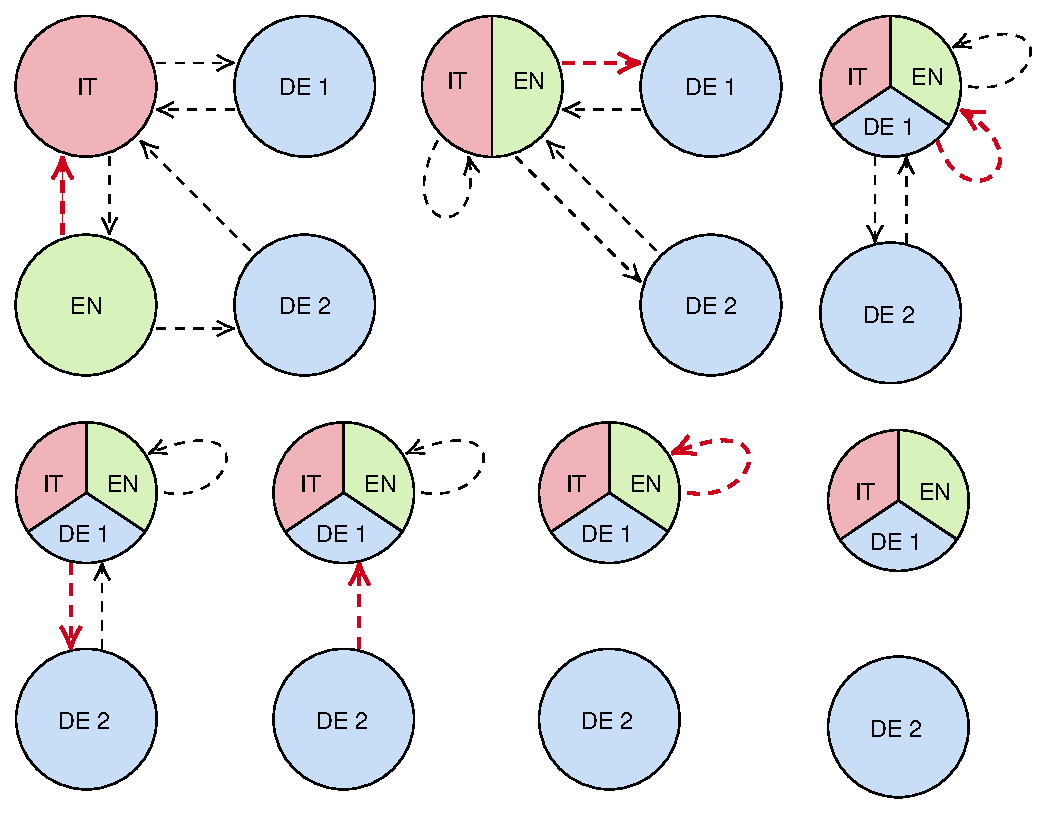
\includegraphics[width=\textwidth]{images/scc_random.pdf}
                    \caption{Here is an example of how four vertices are grouped together when using the \monospace{scc\_random} merging strategy. At each step a random inter-language link is selected and removed from the strongly connected component. Vertices are merged only when the languages they represent do not overlap. If one performs a large number of trials and keeps the most often grouping, the \textquote{best} solution is likely to be found.}
                    \label{scc_random}
                \end{figure}
                
                This merging strategy is quite effective when \(N\) is high: the average result obtained from a large number of trials should be close to the expected value, and will tend to improve as more trials are performed\footnote{Law of large numbers}.
                
                The value of \(N\) should be higher when the expected dimension of strongly connected components is large --- i.e., when a multilingual graph is formed by many different monolingual graphs. Moreover, \(N\) should be high also when large Wikipedia versions are used: they usually contain many inter-language links, thus making the strongly connected component more connected on average. However, high quality Wikipedia versions are expected to be coherent among them: it should be difficult to find components in which two vertices share a common language. In general, setting \(N\) is not an easy task if one wants to keep it low in order to decrease the computational cost: when the value is too low, the chances to have a wrong solution increase; on the other hand, when the value is too high, the computational cost increases rapidly. In each different setting there is a different optimal \(N\) value.
                
                Finally, I want to describe a small but important implementation detail. In particular, I want to focus on two steps of the algorithm presented above: the building of a subgraph using only inter-language links, and the deleting/restoring of inter-language links. An efficient implementation of these parts is possible thanks to the \monospace{graph\_tool.GraphView} class\footnote{\url{https://graph-tool.skewed.de/static/doc/graph_tool.html\#graph_tool.GraphView}.}: it allows to filter out vertices and edges of a \monospace{graph\_tool.Graph} object without the need to create distinct copies of the original graph.